\documentclass[20pt]{beamer}
\usepackage[]{bookmark}
\usepackage[utf8]{inputenc}
\usepackage{amsmath}
\usepackage{amsfonts}
\usepackage{amssymb}
\usepackage{tikz}
\usepackage{xcolor}
\usepackage[dutch]{babel}
\usepackage{sansmathaccent}
\usepackage{graphicx}

\usepackage[style=authoryear,backend=biber]{biblatex}

\addbibresource{bibliography2.bib} 
\pdfmapfile{+sansmathaccent.map}

\title{RMC voor lineaire ODEs}
\author{Isidoor Pinillo Esquivel }
\usetheme{Madrid}
\date{}

\begin{document}

\begin{frame}
    \titlepage
\end{frame}


\begin{frame}
    \frametitle{probleemstelling}
    Numeriek oplossen van
    \begin{equation}
        y'(t)=A(t)y(t) + f(t), \quad y(0)=y_0.
    \end{equation}
    met oog op PDEs
\end{frame}

\begin{frame}
    \frametitle{mijn motivatie}
    Veralgemenen van WoS algoritme van (\cite{sawhney_grid-free_2022})
    naar tijd
    \vspace{-0.25cm}
    \begin{figure}[h!]
        \centering
        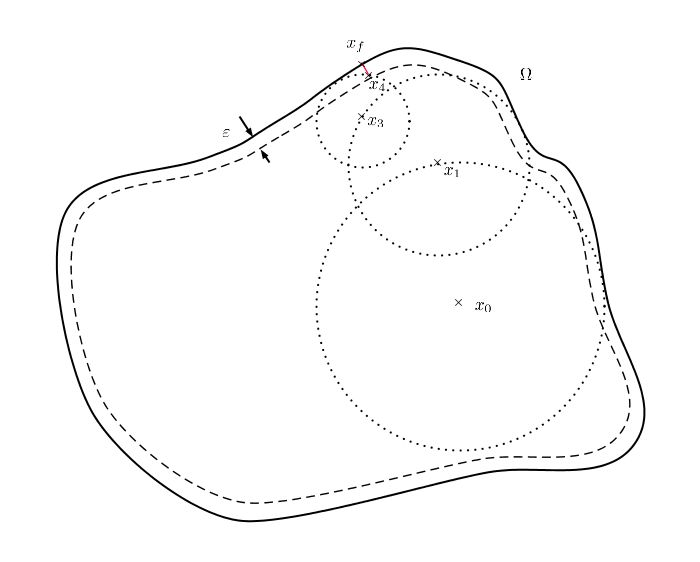
\includegraphics[width=0.6\textwidth]{Walk_on_Spheres_illustration.jpg}
        \label{fig:Walk_on_Spheres_illustration.jpg}
    \end{figure}
\end{frame}

\begin{frame}
    \frametitle{motivatie literatuur}
    - Optimale random convergentie snelheid voor oplossen van IVPs \\
    (\cite{daun_randomized_2011}) \\
    - Veralgemenen van Monte Carlo voor lineaire stelsels (page rank)
    naar IVPs \\
    (\cite{ermakov_monte_2021})
\end{frame}

\end{document}